\documentclass[10pt, oneside]{article}
\usepackage{amsmath, amsthm, amssymb, calrsfs, wasysym, verbatim, bbm, color, graphics, geometry, datetime2}
\usepackage{graphicx}
\usepackage{wrapfig}
% \graphicspath{ {./Template/images/} }
\geometry{tmargin=.75in, bmargin=.75in, lmargin=.75in, rmargin = .75in}

\newcommand{\R}{\mathbb{R}}
\newcommand{\C}{\mathbb{C}}
\newcommand{\Z}{\mathbb{Z}}
\newcommand{\N}{\mathbb{N}}
\newcommand{\Q}{\mathbb{Q}}
\newcommand{\Cdot}{\boldsymbol{\cdot}}

\newtheorem{thm}{Theorem}
\newtheorem{defn}{Definition}
\newtheorem{conv}{Convention}
\newtheorem{rem}{Remark}
\newtheorem{lem}{Lemma}
\newtheorem{cor}{Corollary}


\title{Course name: [Course Code]}
\author{[Javier Perez Tobia]}
\date{Academic Year 2021--2022}

\begin{document}

\maketitle

\begin{figure}[h]\label{fig:cover}
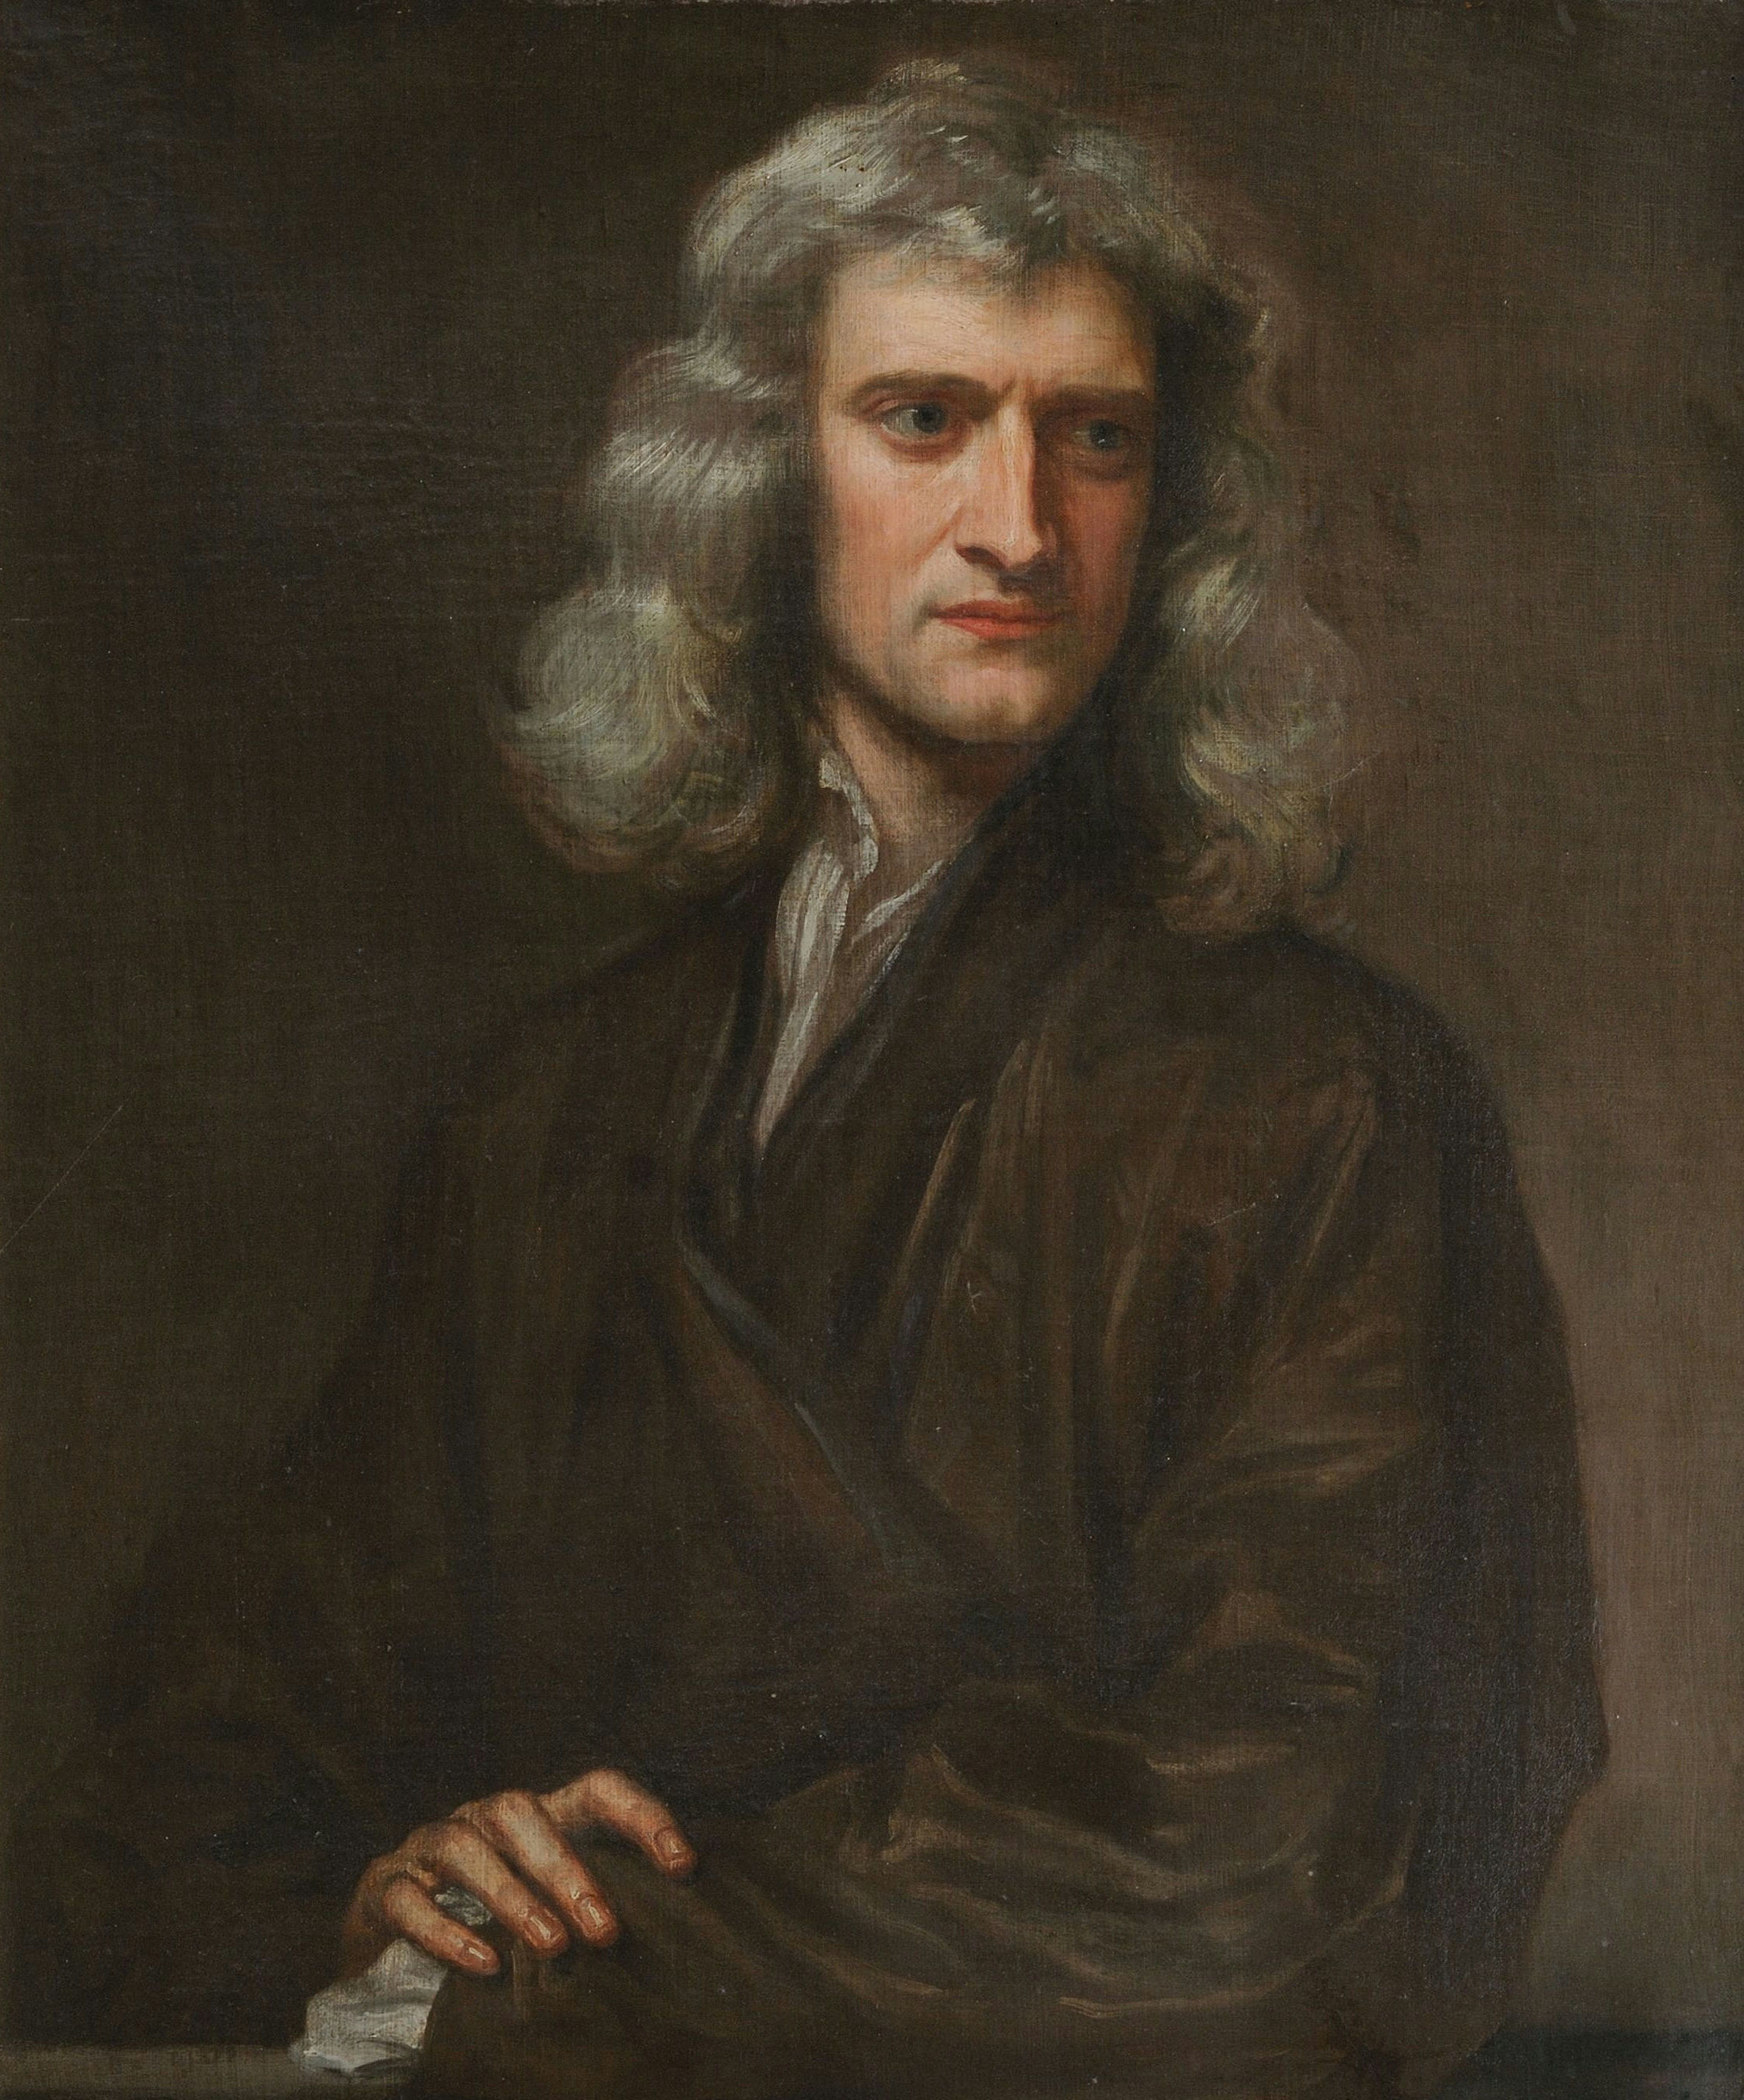
\includegraphics[width=8cm]{./images/newton1}  % {newton1.jpg}
\centering
\end{figure}

\newpage

\tableofcontents

\newpage

\vspace{.25in}

\newpage
\section{Syllabus}\label{sec:syllabus}
\begin{itemize}
    \item Room:
    \item Professor:
    \item Contact:
    \item Schedule:
    \item Exam dates:
    \item Assignment dates:
    \item Grading system:
\end{itemize}

\newpage
\section{Newton's equations of motion}\label{sec:newton's-equations-of-motion}

\subsection{Main equations}\label{subsec:main-equations}
\begin{wrapfigure}{r}{0.25\textwidth} %this figure will be at the right
    \centering
    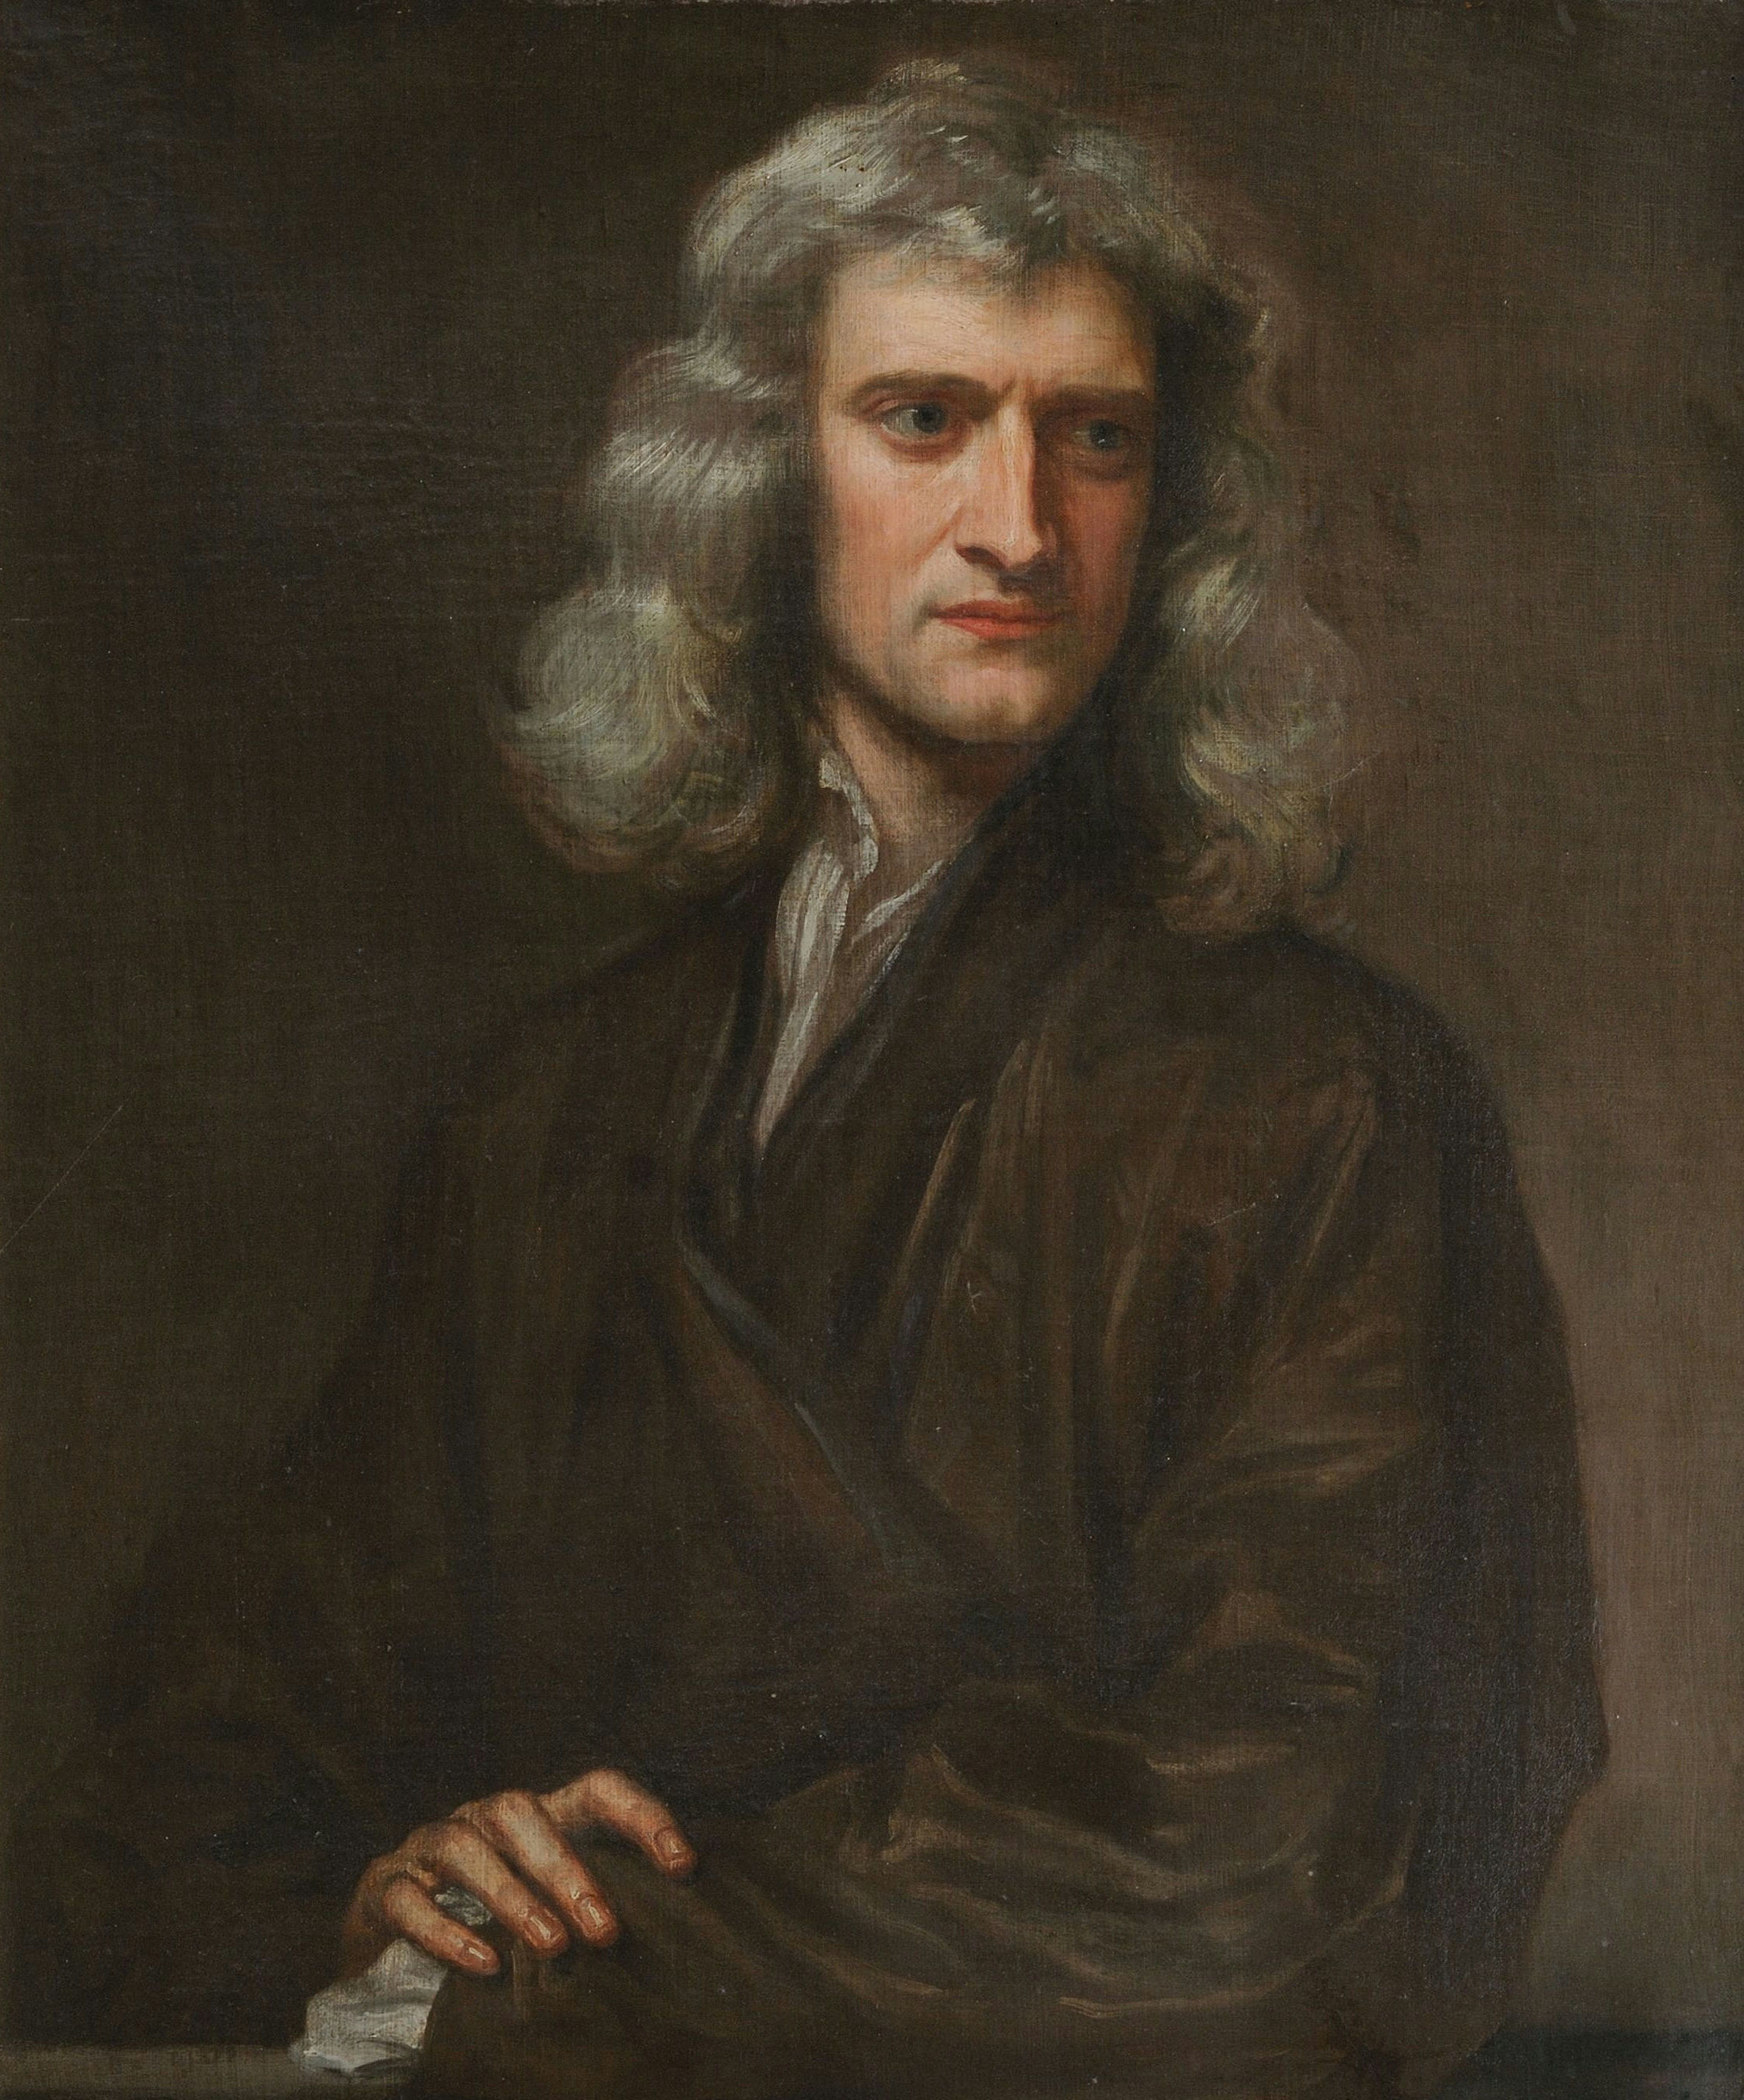
\includegraphics[width=0.25\textwidth]{./images/newton1}
\end{wrapfigure}

\begin{equation}\label{eq:eq1}
    v_{t} = v_{0} + a  t
\end{equation}

\begin{equation}\label{eq:eq2}
    s_{t} = s_{0} + v_{0}t + \frac{1}{2}at^2
\end{equation}

\subsection{Derived equations}\label{subsec:derived-equations}
Now, solving for t in~\ref{eq:eq1} we can derive the following:
\begin{equation}\label{eq:eq3}
    \frac{v_{t} - v_{0}}{a} =  t
\end{equation}
Plugging into~\ref{eq:eq2} we get:
\begin{equation}\label{eq:eq4} \nonumber
\begin{split}
s_{t} & = s_{0}+v_{0}\frac{v_{t} - v_{0}}{a}+\frac{1}{2}a\left(\frac{v_{t} - v_{0}}{a}\right)^2 \\
a(s_{t} - s_{0}) & = v_{0}v_{t}-v_{0}^2 + \frac{1}{2}(v_{t}^2+v_{0}^2-2v_{0}v_{t}) \\
a(s_{t} - s_{0}) & = \frac{1}{2}(v_{t}^2-v_{0}^2) \\
\end{split}
\end{equation}
Finally arriving to:
\begin{equation}\label{eq:eq5}
    v_{t}^2 = v_{0}^2 +2a(s_{t}-s_{0})
\end{equation}

\newpage
\section{Other equation}\label{sec:other-equation}

\end{document}
